\documentclass[a4paper,11pt, oneside]{report}

% Package import
\usepackage[a4paper,inner=3.5cm,outer=2.5cm]{geometry}
\usepackage[english,american]{babel}
\usepackage{fancyhdr}
\usepackage{latexsym}
\usepackage[T1]{fontenc}
\usepackage[utf8]{inputenc}
\usepackage{graphicx}
\usepackage{hyperref}
\usepackage{tabularx}
\usepackage{etoolbox}
\usepackage{fancyhdr}
\usepackage{amsthm}
\usepackage{mathtools}
\usepackage[xindy]{glossaries}
\usepackage{lastpage}
\usepackage{float}
\usepackage{fancyhdr}

\usepackage{listings}
\usepackage{xcolor}

\colorlet{punct}{red!60!black}
\definecolor{background}{HTML}{F7F7F7}
\definecolor{delim}{RGB}{20,105,176}
\colorlet{numb}{magenta!60!black}

\theoremstyle{definition}
\newtheorem{exmp}{Example}[subsection]

\makeglossaries

\setcounter{secnumdepth}{2}
\setcounter{tocdepth}{1}


\lstdefinelanguage{json}{
    basicstyle=\normalfont\ttfamily,
    numbers=left,
    numberstyle=\scriptsize,
    stepnumber=1,
    numbersep=8pt,
    showstringspaces=false,
    breaklines=true,
    frame=lines,
    backgroundcolor=\color{background},
    literate=
     *{0}{{{\color{numb}0}}}{1}
      {1}{{{\color{numb}1}}}{1}
      {2}{{{\color{numb}2}}}{1}
      {3}{{{\color{numb}3}}}{1}
      {4}{{{\color{numb}4}}}{1}
      {5}{{{\color{numb}5}}}{1}
      {6}{{{\color{numb}6}}}{1}
      {7}{{{\color{numb}7}}}{1}
      {8}{{{\color{numb}8}}}{1}
      {9}{{{\color{numb}9}}}{1}
      {:}{{{\color{punct}{:}}}}{1}
      {,}{{{\color{punct}{,}}}}{1}
      {\{}{{{\color{delim}{\{}}}}{1}
      {\}}{{{\color{delim}{\}}}}}{1}
      {[}{{{\color{delim}{[}}}}{1}
      {]}{{{\color{delim}{]}}}}{1},
}

% clear default
\fancyhead{}
\fancyfoot{}

\usepackage{fancyhdr}
\pagestyle{fancy}
\fancyhf{}
\renewcommand{\headrulewidth}{0pt} % optional
\fancyfoot[L]{Chapter: \nouppercase{\leftmark}}
\fancyfoot[R]{\thepage/\pageref{LastPage}}

% Redefine the plain page style, Chpater page
\fancypagestyle{plain}{%
  \fancyhf{}
  \renewcommand{\headrulewidth}{0pt} % optional
  \fancyfoot[R]{\thepage/\pageref{LastPage}}
}

\renewcommand{\chaptermark}[1]{\markboth{\MakeUppercase{#1}}{}}


% URL Line breaks
\makeatletter
\g@addto@macro{\UrlBreaks}{\UrlOrds}
\makeatother

\begin{document}


\pagestyle{empty} %Keine Kopf-/Fusszeilen auf den ersten Seiten.
\begin{titlepage}
\begin{center}

% Oberer Teil der Titelseite:

\includegraphics[width=0.08\textwidth]{img/bfh_logo.png}\\[1cm]    
\textsc{\LARGE Bern University of Applied Sciences}\\[1.5cm]
\textsc{\Large Informatics Seminar}\\[0.5cm]

% Title
\newcommand{\HRule}{\rule{\linewidth}{0.3mm}}
\HRule \\[0.4cm]
{\huge InterPlanetary File System}\\[0.3cm]
{\huge \bfseries  IPFS}
\HRule \\[1.5cm]

% Author und Lehrer
\begin{minipage}{0.4\textwidth}
\begin{flushleft} \large
\emph{Author:}\\
Martin \textsc{Schmidli}\\
\end{flushleft}
\end{minipage}
\hfill
\begin{minipage}{0.4\textwidth}
\begin{flushright} \large
\emph{Teacher:} \\
Kai \textsc{Brünnler}
\end{flushright}
\end{minipage}
\vfill


% Unterer Teil der Seite
Bern, {\large \today}
\end{center}
\end{titlepage}
\pagestyle{fancy}

\tableofcontents


\chapter{Abstract}
%https://github.com/ipfs/ipfs, Overview
IPFS (InterPlanetary Filesystem) is an opensource protocol which can be used to run a distributed filesystem. IPFS was invented to tackle the drawbacks of the Internet and the Internetprotocol suite we are using today.\\  \\
To understand why IPFS was invented, we first have to understand the issues we have today. This report will outline how IPFS works, what kind of issues it tries to resolv and analyze the obstacles which have to be overcome to establish IPFS as a accpted and widely used technology.

\chapter{Introduction}
IPFS stands for InterPlanetary Filesystem. It's an opensource Internet Protocol which can be used to run a distributed filesystem.
The developers didn't invent IPFS from scratch. In its core IPFS takes advantage of existing ideas like Kademlia DHT, BitTorrent and Git. The main intention behind IPFS is to tackle the issues  we are having in todays Internet/Web. In the eyes of the inventors the protocol should be seen as an upgrade or even as a replacemnet of the existing technolgies like HTTP. Global data distribution should be simplified and be implemented in the protocol itself rather than prescribe a separate distribution mechnism \cite{IPFSBasics}.\\ \\
All computers participating in an IPFS Network are called peers or nodes. IPFS is a peer 2 peer system, there are no central servers managing the network.

\section{Origin}
The Development of IPFS was started in 2014 by Juan Benet, former Stanford Student and founder of the company Protocol Labs . Protocol Labs and contributors of the Community are developing IPFS further \cite{LinkedIn}.

\section{Name}
The name was choosen as a tribute to J. C. R. Licklider, a computer scientist who came up with an idea of a ''intergalactic network'' of computers in 1962 \cite{Tribute}. He imagined a global network of computers, able to talk to each other and exchange data. During his time working at DARPA (Defense Advanced Research Projects Agency) he influenced many peoble with his ideas. DARPA later startet the ARPANET Project and laid the foundation stone for todays Internet. Many important technologies for example: TCP/IP where invented or funded during this project \cite{JCR}. 

\newpage
\section{Project state}
%https://github.com/ipfs/ipfs#overview, Currrent State of IPFS
As of 19.04.2017 the Specifications of the IPFS Protocol are still being developed and hasn't completed yet. The developers state, that the
core parts of the specs have reached a reliable or stable state. No official RFC request have been submitet. An Implmenetation of the Protocol, written in the programming language Go and some utilities have aready been published. Implementation in other programming languages Javascript and Phyton are in developing \cite{specs}.\\ \\
Different sources state different facts how the system will works. Many topics are still discussed intensively. This makes it very difficult to do a report about IPFS. The main data source of this report was the projects github page and a whitepaper release by Juan Benett.

\section{Knownledgebase}
To understand the following chapters you should get yourself familiar with
\begin{itemize}
\item Distributed Hashtables
\item Bittorrent
\item Public-key cryptography 
\end{itemize}

\newpage
 
\chapter{Adressing}
\section{Content Adressing}
Compared to HTTP where data is adressed by URL's is IPFS the data is adressed by its contents hash.\\
To understand how the data adressing in IPFS works, first a little example how its done with HTTP.
\subsection{HTTP}
Data which is access by HTTP is adressd with its hostname, port, path and the filename or searchword \cite{HTTPAdressing}.
\begin{exmp} URL scheme used for HTTP
\noindent
\begin{center}
http : // hostname [ : port ] / path [ ? searchwords ]\\
https://raw.githubusercontent.com/github/gitignore/master/TeX.gitignore
\end{center}
\end{exmp}
\noindent
If the location of the file changes and no redirection was created, the link gets useless.
\noindent
\newpage
\subsection{IPFS}
Data added to the global IPFS can be adressed by the hash of its content. Every time we add data the hash will be calculated. When the content of the file changes the hash will be changed as well.  The older content will still be accessible with the old hash value. The link is immutable, this garanties the persistance of the data.
\begin{exmp} IPFS Link
\begin{center}
	/ipfs/QmbYzb3nScopAnfkoUpRWUFVv856uSWpSRc2KYM1FSBJxr
\end{center}
This scheme has been built similar than unix filesystem paths. This design choice makes it possible to mount the IPFS filyesystem directly into a Unix System. The IPFs filesystem can then be used by applications running on the unix machine.\\ \\
The system is activly deduplicating data. If existing contents gets added for example two times the same picture they will get the same hash value.
\end{exmp}

\newpage

\chapter{Multiformats}

Multiformat is a collection of protocols / formats. They try to extend existing formats by adding self describing components.  Two multiformats which are used in IPFS are Multihash and Multiaddr. This chapter will give you a short introduction to these formats. To understand these formats is necessary as they are used everywhere in the IPFS project.

\section{Hash functions - Multihash}
Multihash is a protocol / format  invented and maintened by the company Protocol Labs. Multihash defines a hash format, which is used in the IPFS project to encode Hashes. Every hash generated will be stored with two addidtional values; the Functioncode of the  hash function, which was used to generate this hash and the length of the hash.
\begin{center}
	Multihash Format = Hash Function Code + Hash Length + Hash
\end{center}
The hash functioncodes were set by the developers. For your own projects you can easily implement your own code hashfunction reference list.\\[0.3cm]
\begin{figure}[H]
\centering
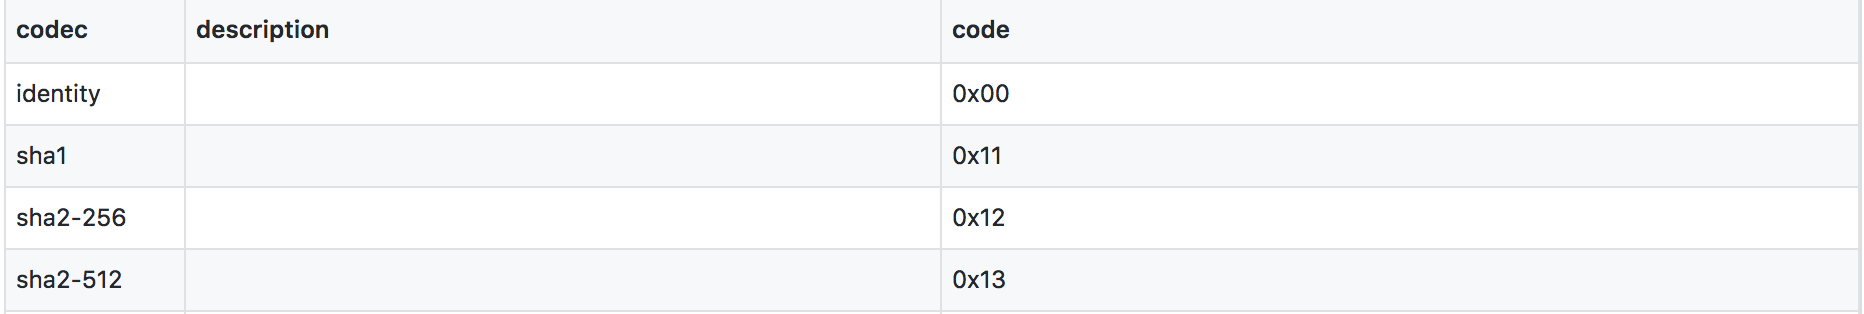
\includegraphics[width=\textwidth]{img/multiformat_hashfunctionid.png}
\caption[Hashfunction code list]{Hashfunction code list}
\end{figure}
\noindent
Multihash should allow the software using IPFS to upgrade the hash functions more easily \cite{multihash}. For example we hardcoded SHA1 as a hash function into our programm. If somebody would be able to break the SHA1 hash function we would have to replace the hash function. This would lead to longer hash values which might break our programm. By using a more generic format the hashfunction can be switched very quickly.\\ \\
By default IPFS Nodes are using sha2-256 as hash function. If a multihash has been generated it will be encoded by Base58 \cite{Encoding}.

\begin{exmp} sha1
\begin{center}
	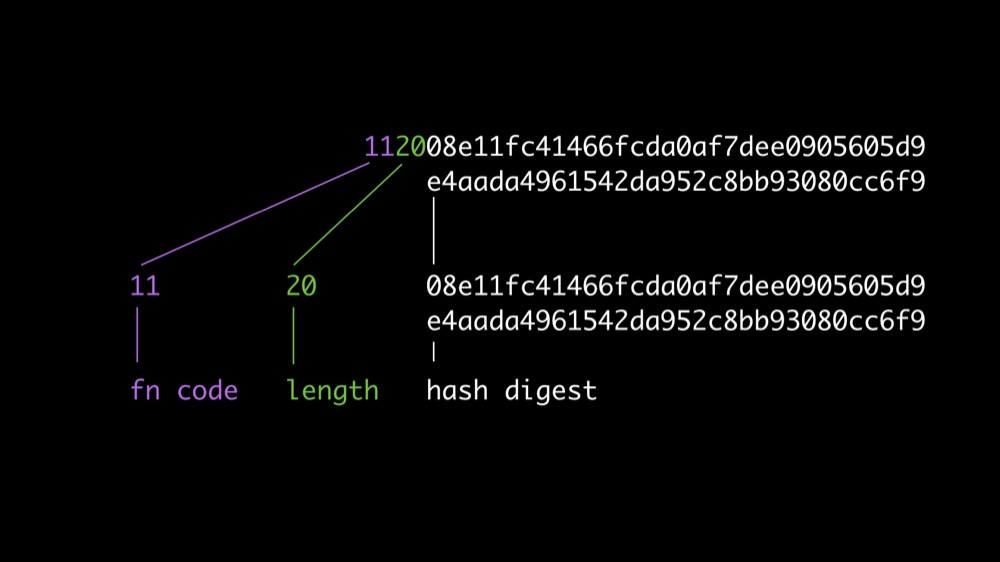
\includegraphics[width=\textwidth]{img/multihash_example.jpg}
\end{center}
\textbf{Functioncode:}\\
0x11, when we lookup the Multihash Function Table we can find \textbf{sha1}. This hash was generated by the sha1 hasfunction.\\ \\
\textbf{Length:}\\
0x20 = 32, means 32 * 8 Bit = 256bit. The Hash is 256bit long.\\ \\
\textbf{Hash Digest:}\\ Hash Values 
\end{exmp}

\newpage

\section{Peer Adressing - Multiaddr}
Multiaddr is used to represent common network adresses in a different way.
\begin{exmp}
Normal representation of a websocket url: 
\begin{center}
ws://1.2.3.4:5678\\
\end{center}
Multiaddr address:
\begin{center}
/ws/1.2.3.4/tcp/5678
\end{center}
\end{exmp}
\noindent
Like in Multihash were every hash function has a function code, in Multiaddr every protocol has a function code. \\
\begin{figure}[H]
\centering
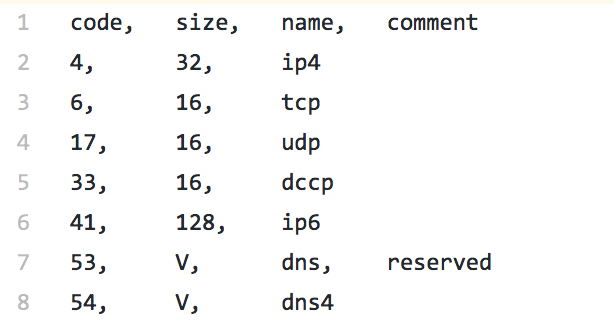
\includegraphics[width=0.6\textwidth]{img/multiaddr.png}
\caption[Multiaddr code list]{Multiaddr code list}
\end{figure}
\noindent
With this change of the format and the substitution of the protocol string by a function code, the hole adress takes up less space in the binary format.
\begin{center}
<1 byte ws code><4 byte ipv4 addr><1 byte tcp code><2 byte tcp port>
\end{center}
\newpage

\chapter{Layer-Architecture}
IPFS is made of a stack of different software moduels / libraries.\\ \\
\noindent
\begin{tabularx}{\textwidth}{XXXl}
Protokoll / Library&Level & Layer & Function\\ \hline
&6& Applications & \\ \hline
IPNS  &5 & Naming & \\ \hline
IPLD&4 & Merkle DAG &\\ \hline
libp2p&3 & Exchange & exchange data blocks\\ 
&2 & Routing  & data lookup\\
&1 & Network  & connect to other nodes \\ \hline
\end{tabularx}\\[0.2cm]
This chapter will guide you from the bottom of the stack to the top to explain in detail how IPFS works.
\section{libp2p - network, routing, exchange}
During the development of IPFS the team learned how hard it was to run IPFS on many different devices with different requirements to the network \cite{libp2pissues}. It was impossible for them to provide one single protocol to work everywhere. They startet to redefine the network, routing and exchnage layer and created a lindependet ibrary call libp2p. This library is responsible for the network connectivitiy between nodes, the data lookup on the network and the data block exchange among them. In its core libp2p basically is a collection of p2p protocols and defines interfaces to use them. There are many different protocols supported which can be used depending of the situation of the node and it's network. The protocols are implemented like blocks and can be combined dependent of the needs of the application developers.
\begin{figure}[H]
\centering
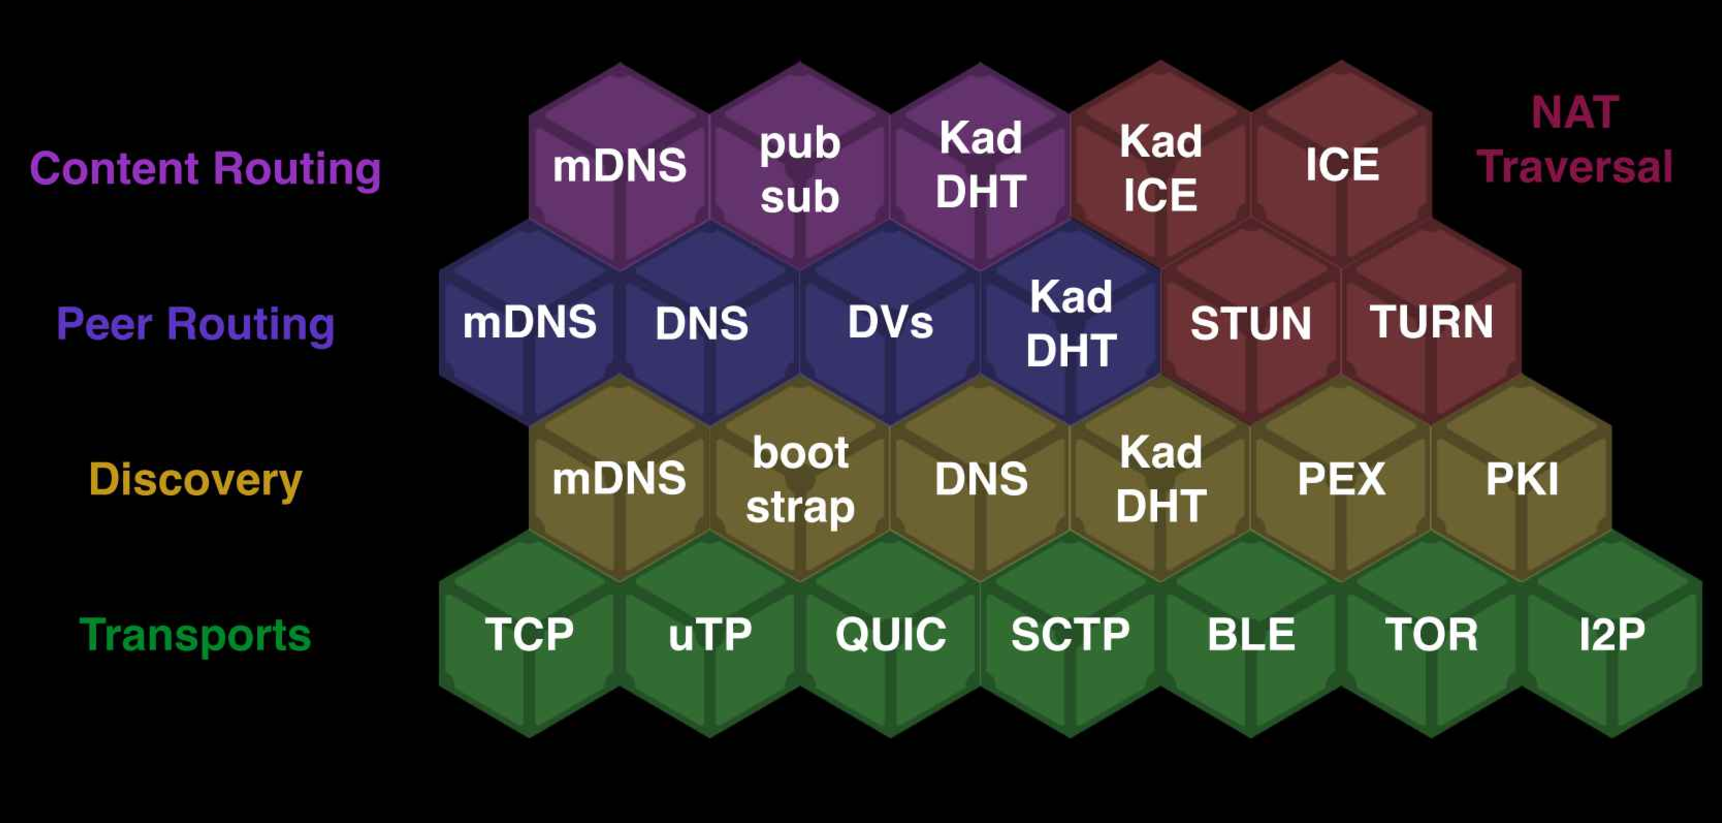
\includegraphics[width=\textwidth]{img/libp2p-blocks.png}\\[0.8cm]
\caption[libp2p]{libp2p protocol collection. Not all are implemeted yet}
\end{figure}
\noindent
\subsection{Network}
libp2p has been designed to be transport independen. It can run without IP stack for example on NDN, XIA and Bluetooth\cite{libp2pnoip}.\\ 
libp2p doesn't determine which kind of protocol should be used. For every layer the developer is responsible to chose which protocols he would like to implement. Witch this choice, the developer decides how his application will work with other applications on the network.\\ \\
For example if the developer decides to route the data over the TOR (the onion router) network the application will not be able to exchange data with nods within the same network. It's a tradeoff, the application will be more secure, as it benefits of the anonymity of the TOR network but you will give up performance. 

\begin{figure}[H]
\centering
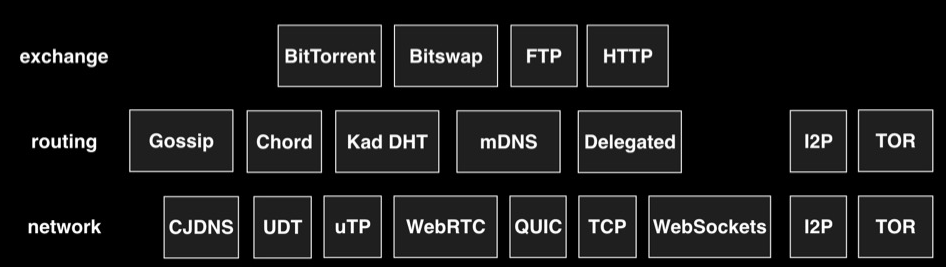
\includegraphics[width=\textwidth]{img/libp2p-protocols.png}\\[0.8cm]
\caption[libp2p]{libp2p protocols.}
\end{figure}
\subsection{Routing}
This part of libp2p gives the ipfs node the ability to find the network adress of other nodes and nodes which can serve specific data blocks.  The peer routing module takes in a key (hash) and responds with one or more Peer Info Objects. The Peer Info contais the PeerID and its multiaddr adresses. Whith these informations the other node can be contacted.\\ \\
The system is easily expandable. The protocls just need to fullfill the requirements of the Peer Routing interface. Currently there are two Routing systems proposed and implemented.\\ \\
Every node in a routing system can contact all the participating peers. If data should be separated from the the public IPFS network a separate instance of a routing system needs to be established. For example: create your own DHT.

\subsubsection{Kadmelia DHT}
A Kademlia distributed hash table can be used to store Key Value pairs.\\ \\
If a IPFS Node adds new data to the network, the hash of the data (key) is added to the DHT plus its own Peer Info (value). This process is called providing \cite{dht-provide}. If a node wants to find out where he can get the specific data blocks, it can use the DHT to determine the nodes which can serve those blocks.

\subsubsection{mDNS}
Uses the mDns protocol to check if a node in the local network holds a specific key.

\newpage
\subsection{Identities}
During the initialization of a node, a 2048-bit RSA keypair (public, private) is generated. A hash function is used to generate the hash of the public key. This generated hash is then used as Peer ID \cite{PeerID}.
\begin{center}
Peer ID = multihash(public key)
\end{center}

\subsubsection{Trust}
There is no central certification authority in place which can be used to check if another peer can be trusted. The hole system has been designed to be self-verifing.\\[0.3cm]
\begin{exmp} Communication\\ \\
Peer A contatcs another peer B. The Nodes exchange Node ID and Public Key.
Peer A generates the hash of the public key of peer B. If this generated hash doesn't mach the NodeID of peer B the connection will be terminated.\\[0.3cm]
\begin{figure}[H]
\centering
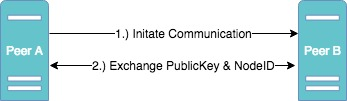
\includegraphics[width=0.6\textwidth]{img/ipfs_peertrust_scenario_init.jpg}\\[0.8cm]
\caption[Node trust]{Node trust setup}
\end{figure}
\end{exmp}
\newpage
\begin{exmp}  Attack scenario\\ \\
Peer C tries to steal the identity of peer A. Peer C is using the public key and the Node ID from peer A . Peer B will establish a connection with peer C as the public key is valid and the Node ID matches. The sent data from B to C will be encrypted by Peer A's public key. As Peer C doesnt hold the private key, the data can't be decrypted and therefor its useless.
\begin{figure}[H]
\centering
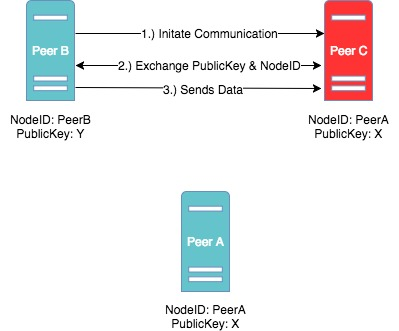
\includegraphics[width=0.6\textwidth]{img/ipfs_peertrust_scenario_attack.jpg}\\[0.8cm]
\caption[Node trust attack]{Node trust attack}
\end{figure}
\end{exmp}

\newpage

\newpage
\section{Exchange - Bitswap}
Many exchange protocols can be used with IPFS for example FTP, HTTP, Bittorrent or Bitswap.\\ \\
Bitswap is a bittorrent-inspired software module used to exchange data blocks between the nodes of the IPFS network. When a user requests a piece of data the specific blocks are added to the nodes ''want\_list'' list. Bitswap contacts other peers which own the data according to the Routung system (example. DHT) and sent them the ''want\_list''. Peers keep track of the blocks which they own by putting them into their ''have\_list'. If the reciever has blocks which another node requested, he will send the blocks back to the requester. 'When the blocks arrive, the requester will imidiately send out a ''Cancel' signal. Other nodes will stop sending those blocks. After the blocks arrived the requester move those blocks from the want\_list to the have\_list  \cite{bitswap}.

\subsection{Exchange Strategies}
When a bitswap node requests data (Peer A), the other nodes (Peer B) will only send the requested data if they recieve blocks in return. Most of the time Nodes store very different data and the amount of blocks which they could offer in return is very limited. Sometimes Node don't own any data the other node is needing. This puts the requesting node (Node A) in a bad position as it has nothing he could offer in exchange. To resolve the situation, Node A will start to download the data Node B has on its want\_list  after all his own data requestes are completed.  The own needs have a higher priotity.\\ \\

\newpage
\begin{exmp}
Let's make a short example of how this strategy works.\\ 
We have 3 Nodes, A, B and C. Node A wants blocks of a ''music file'' but currently the Node doesn't store any data. Node B want's blocks of a ''science paper'' file and owns blocks of the ''music file''$\rightarrow$ Node A has no blocks which Node B actually needs.
\begin{center}
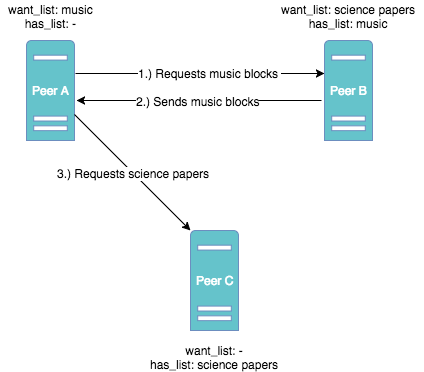
\includegraphics[width=0.7\textwidth]{img/ipfs_bitswap_noblocks.png}\\[0.3cm] 
\end{center}
After Peer A got all the music blocks he wanted, he will start to look for science paper blocks.
\end{exmp}

\subsection{Ledger}
Bitswap nodes keep track of the amount of data they send and received to other nodes in a digital ledger. We speak of credit or dept between the nodes. It's an indicator of the trust and the connection between two nodes. When a new connection is established, the nodes exchange their ledger. If the ledger data doesn't match, for example if one of the nodes  maliciously changed the data, the ledger and the connection will be resetet. Depending of the Bitswap strategy good connections between nodes, which already exchange alot of data could be prefered. Nodes with a high dept could be neglected.

\newpage
\subsubsection{Automatical Download Problematic}
This exchange mechanism leads to data download even if the node doesnt actually need the data by itself. The data are cached and increase the availability of the blocks. This strategy is not yet implemented in bitswamp. Todays implementation is syncing blocks without any conditions and doesn't fullfills the defined protocol specifications.\\ \\ 
There are ongoing discussions if this feature should be enabled by default or if there should be a config a option to enable it \cite{bitswapstrategy}. If this feature is enabled by default, IPFS nodes would download data without any knowledge of the user. This would lead to a extensive usage of the local storage and could lead to legal problems. To avoid the legal problematic, there need to be a system in place to avoid the download of Copyright Protected Data and to implement Digital Right Management (DRM). If and how this will be implemented is currently discussed in the community \cite{copyright}. Some possible approches which are considered are 
\begin{itemize}
\item White, Blacklist of certain blocks and objects\\ Users can enable filters which kind of content they want to download
\item Public trusted list of Copyright Protected content. \\ Prohibits the sharing of files on this list
\end{itemize}


\subsection{Data Availabiliy}
In todays implementation of IPFS, data is not actively distributed in the IPFS Network. If a node requests data, it will be downloaded and therefore replicated. There is no higher instance which is controlling how many times a specific data block is physicaly stored somewhere. Example; If one data block is added from Node A to the IPFS network and this node goes down, the data is no longer available.\\ \\ The developers try to solve this problem by designing a new software which is running on top of IPFS called IPFS-Cluster. The IPFS-Cluster Service will be running on the IPFS Node and makes sure, that data remains available. If data is clustered its ''pinned'' to a Node. Data will be replicated/pinned among IPFS-Cluster nodes accoring to a predefined replication factor. Example; Replication factor 2, data us store on 2 Nodes. If a node with pinned data goes down, the data automatically is replicated to other cluster nodes.

\subsection{Difference to Bittorrent}

Bittorrent nodes can only request blocks from one torrent. Data blocks are not shared among torrents.

%https://www.youtube.com/watch?v=9UjqJTCg_h4


\newpage

\section{IPLD - Merkle DAG}
IPLD stands for Inter Planetary Linked Data. IPLD defines
\begin{itemize}
\item Merkle directed acyclic graph\\ Used to create a relationship between the IPFS objects added to the DHT. The Merkle DAG gives a structure to the loose objects in the DHT / Routing System.
\item Merkle links \\ Edges /links  between the objects of the DAG
\item Merkle paths \\ Unix like path for traversing through the merkle dag
\item IPLD Data Model \\ Defines the data structure of the DAG objects, based on the JSON format
\end{itemize}

\subsection{Merkle DAG \& Merkle Links}
A Merkle DAG is a Directed Acyclic Graph where the objects are conected with merke-links. The Merkel DAG has the follwing features:
\begin{itemize}
\item No cicle is allowed
\item Content is adressed by hashes $\rightarrow$  merkle-link\\ \\
Example:  /ipfs/QmKLTg7BZ ... 63JtDuvs2k\\ \\
Using merkle-links provides some advantages
\begin{itemize}
\item Accessed data can be verified / integrity checked by the hash.  
\item data structures can't be modiefied as a change results in a new hash.
\end{itemize}
% \item When data is added to the graph it is automatically verified with the contents hash
\item Data will be stored only once in the DAG, if data is added twice it will be reference by its hash $\rightarrow$ Automatic deduplication
\end{itemize}
The Merkle DAG Datastructure is different than a Merkle Tree. The Merkle DAG doesnt need to be balanced, the added data is automatically dedublicated and all nodes can contain data whereas in a Merkle tree only leaf nodes can contain data.

\newpage

\subsection{IPLD Data objects}
IPLD defines a basic datamodel based on JSON. The objects can be structured by the developer. This makes the DAG very flexibel. Various objects can be modelled to create compley datastructures.

\subsubsection{Merkle Links}
A merkle-link object contains of a key ''/'' which defines a link to another object and the actual link value. The link value can be a multihash or the absolut path with the ''/ips'' präfix. 
\begin{lstlisting}[language=json]
{ "/" : "/ipfs/QmKLTg7BZ ... 63JtDuvs2k" }
\end{lstlisting}

\subsubsection{Objects}
IPLD objects are basic JSON objects. They can be linked with merkle-links.
\begin{lstlisting}[language=json]
{ "name": "Martin Schmidlli" }
\end{lstlisting}

\begin{exmp} Example of linked objects
\begin{figure}[H]
\centering
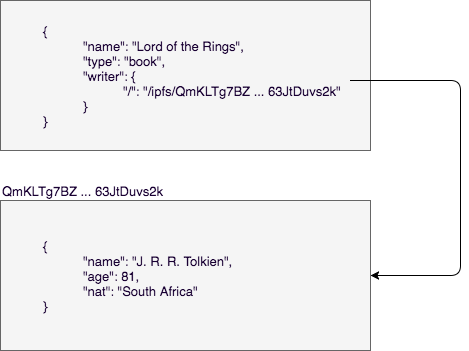
\includegraphics[width=0.7\textwidth]{img/ipld-example.png}\\[0.8cm]
\caption[IPLD linked objects]{IPLD linked objects}
\end{figure}
\end{exmp}

\subsection{Merkle Paths}
This is our basic object at the link /ipfs/QmKLTg7BZ ... 63JtDuvs2k\\
\begin{lstlisting}[language=json]
{ level1 : {
	level2: "Hello World"
}}
\end{lstlisting}
We can use merkle paths to reference to value or another objects relative to the root.
\begin{center}
/ipfs/QmKLTg7BZ ... 63JtDuvs2k/level1/level2
\end{center}
We can traverse through the DAG Object /ipfs/QmKLTg7BZ ... 63JtDuvs2k like in a unix filesystem and access values of level2.
\begin{exmp} ipld cat
\begin{lstlisting}[language=json]
> ipld cat --json QmKLTg7BZ ... 63JtDuvs2k/level1/level2
"Hello World"
\end{lstlisting}
\end{exmp}


\subsection{Small Files <= 256kB}
If the added data is smaller than 256kB, it's is stored directly into the DAG Object.
\begin{figure}[H]
\centering
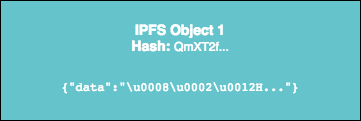
\includegraphics[width=0.6\textwidth]{img/ipfs-fileblocks-small.png}
\caption[Small Object]{Small Object <= 256kB}
\end{figure}

\newpage
\subsection{Large Files > 256kB}
If we add a file bigger than 256kB, the file will be split up into blocks. The generated hash will be the root node in the DAG. This root node will contain merlkle-links to the subblocks / objects. The data segment is used to declare that this object represents a big file.\\ \\
If a node requests a block, this block can come from any node owning one of these blocks even if its not from the same ''file'' \cite{fileblock}. Mutlible IPFS objects can share blocks. As IPFS is adressed by hash, the actual data block is stored once.\cite{fileblock2}. \\[0.3cm]
\begin{figure}[H]
\centering
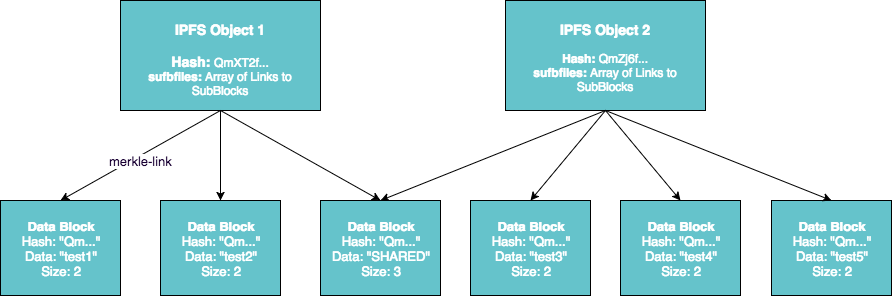
\includegraphics[width=\textwidth]{img/ipfs-fileblocks-big.png}
\caption[Big Object \& Blocks]{Abstract visualization how blocks are handeled}
\end{figure}

\newpage
\begin{exmp}Add a large File to IPFS \\
\begin{figure}[H]
\centering
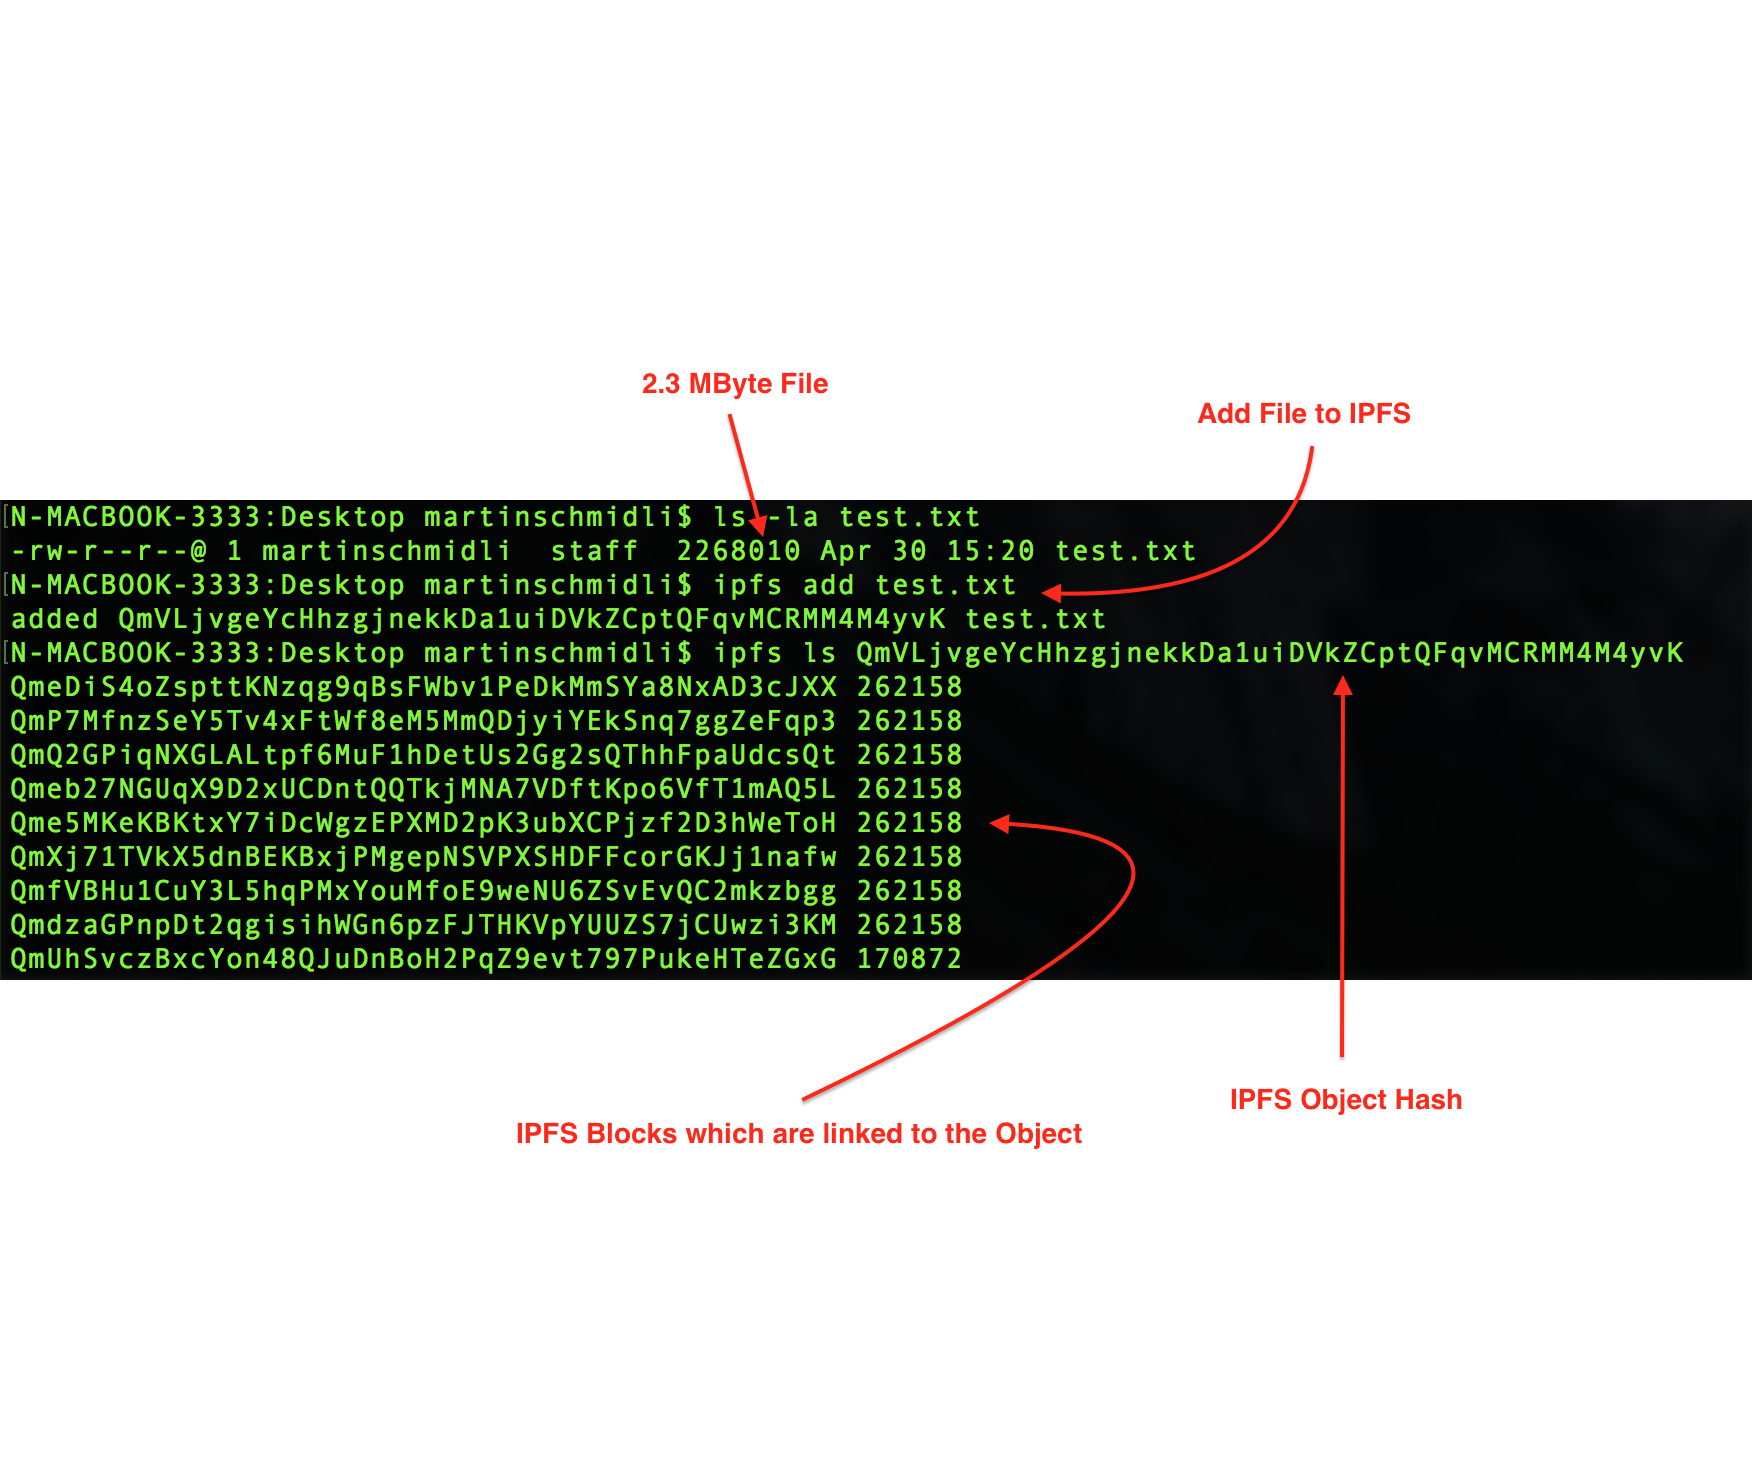
\includegraphics[width=\textwidth]{img/ipfs-object-example.png}
\caption[IPFS Objects Example]{Add a big IPFS Objects}
\end{figure}
\end{exmp}

\subsection{Encryption}
Built-in file level encyption is one of the many missing features in IPFS today. The feature is listed in the IPFS whitepaper and will be added in a later release of the protocol. \cite{Encryption}. Data added to the IPFS network will automatically be encrypted. If private data is added to the ''public'' IPFS network, the developers recommend to encrypt it manually \cite{EncryptionManual}.

\newpage
\subsection{Complex Datastructures}
The basic DAG objects can be used to build more advanced datastructures. Till today there are many implementations already developed:
\begin{itemize}
\item git
\item Zcash (crypto currency)
\item Bitcoin /crypto currency)
\item Ethereum
\item Unix Filesystem
\end{itemize}
\begin{exmp}IPFS Directory
\begin{figure}[H]
\centering
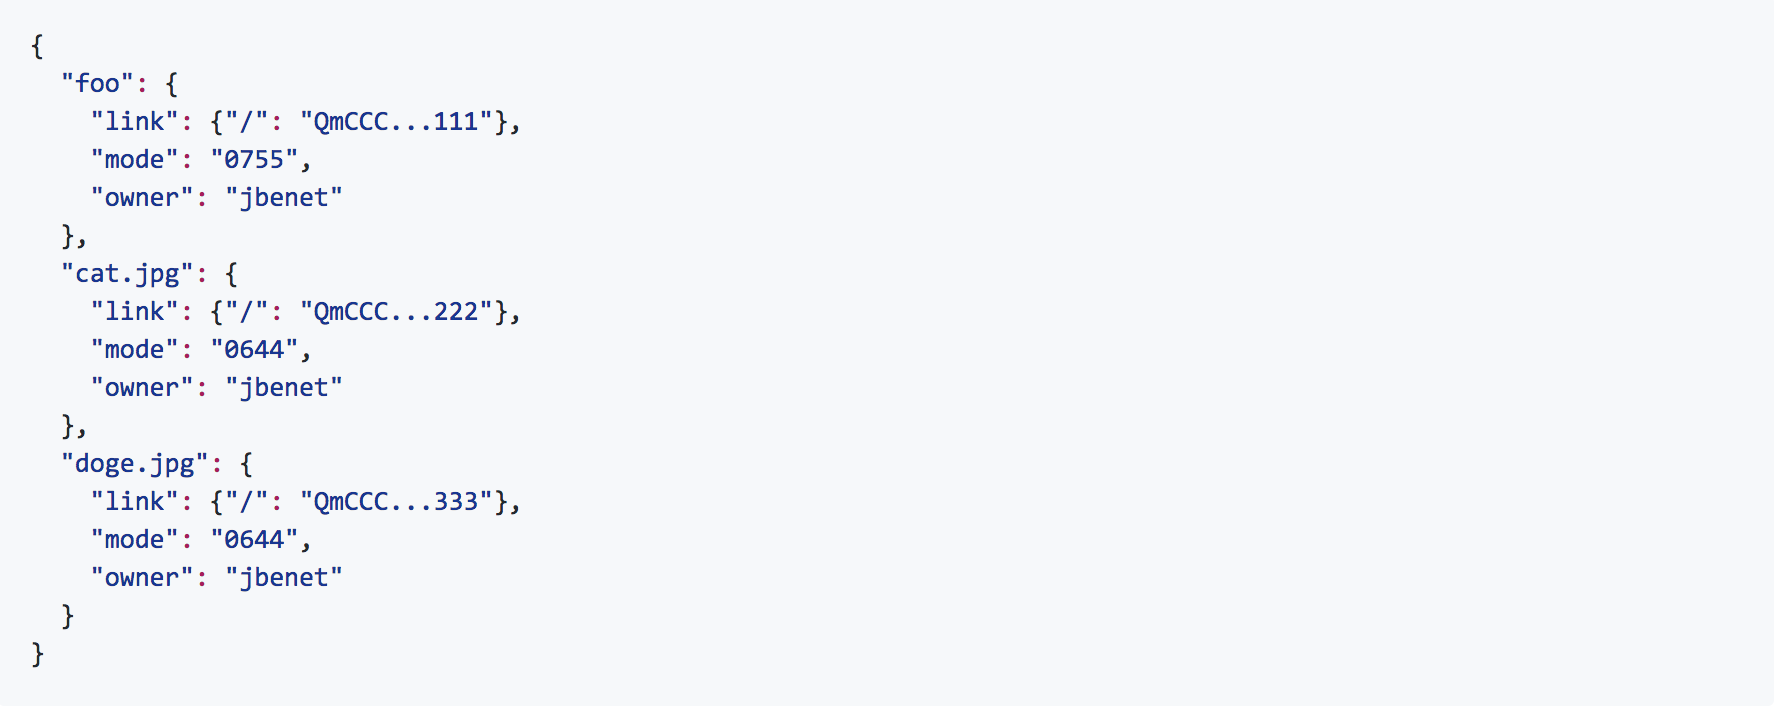
\includegraphics[width=\textwidth]{img/dag-object-dir.png}
\caption[DAG Directory]{DAG Objects - Directory}
\end{figure}
\end{exmp}
\newpage
\begin{exmp}IPFS Git commit message
\begin{figure}[H]
\centering
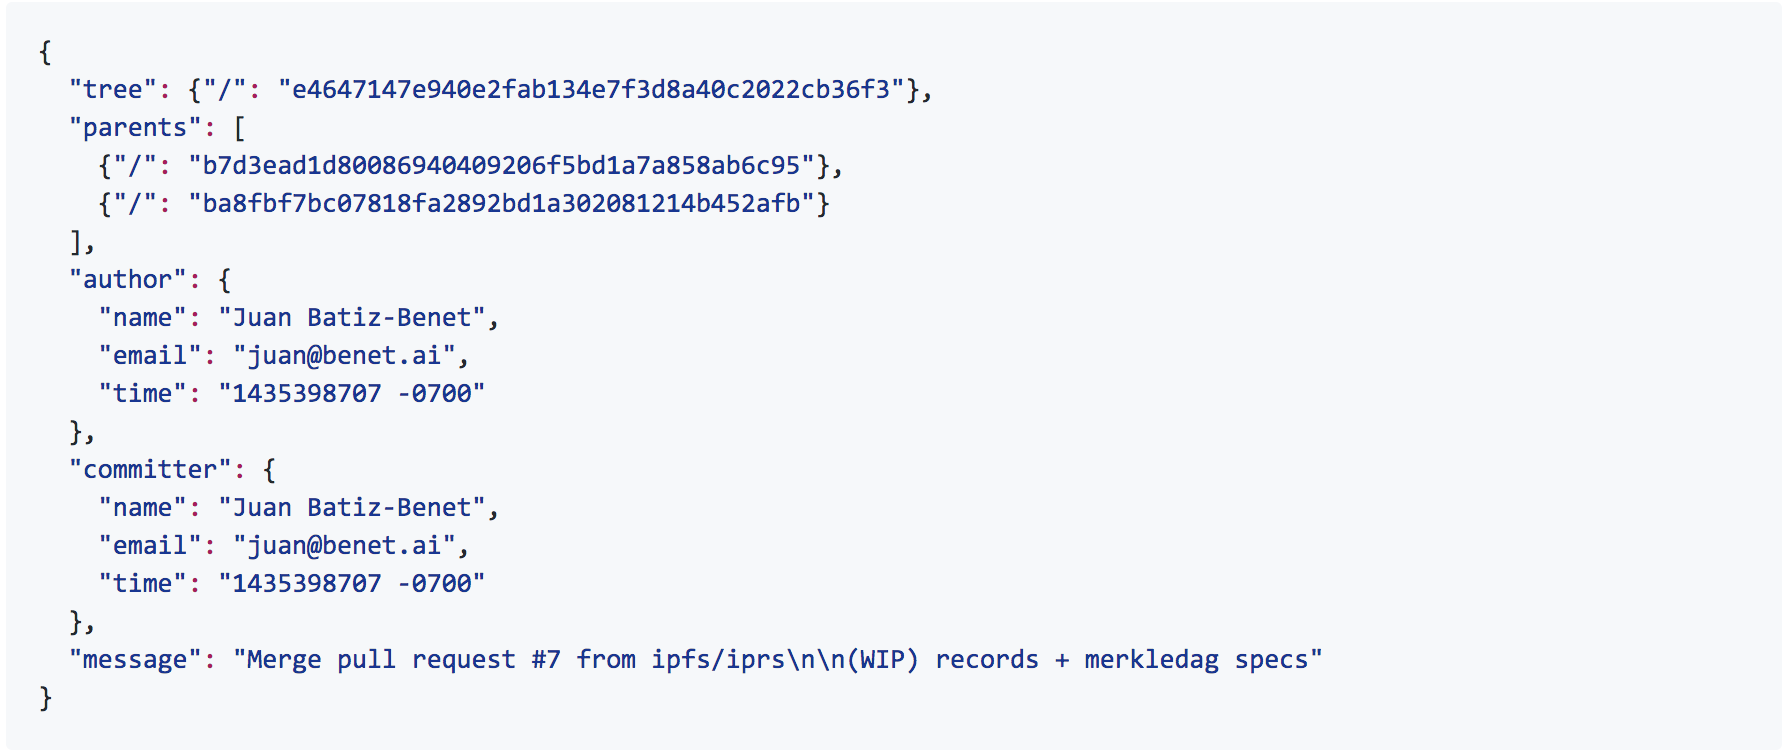
\includegraphics[width=\textwidth]{img/dag-object-gitcommit.png}
\caption[DAG Objects commit]{DAG Objects - Git commit}
\end{figure}
\end{exmp}
\begin{exmp}IPFS Bitcoin block
\begin{figure}[H]
\centering
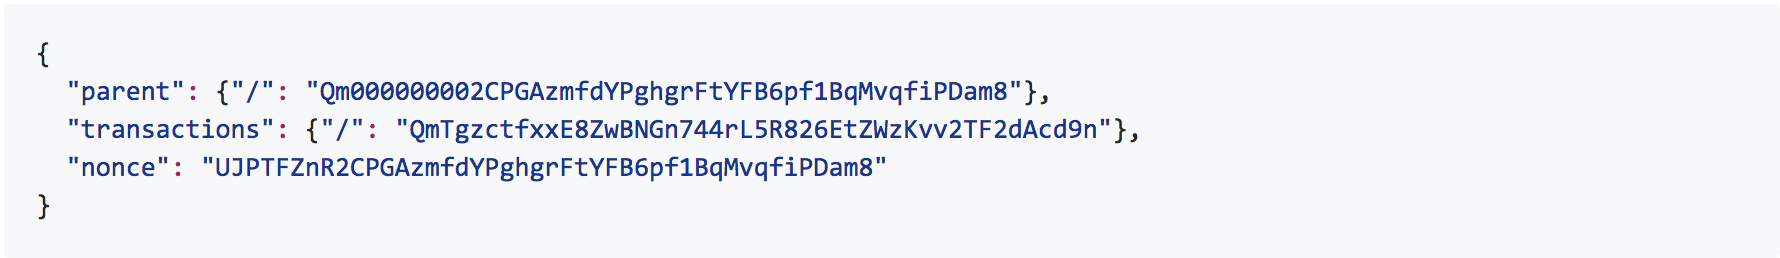
\includegraphics[width=\textwidth]{img/dag-object-blockchain.png}
\caption[DAG Bitcoin block]{DAG Objects - Bitcoin block}
\end{figure}
\end{exmp}

\newpage
\section{State Mutability - IPNS}
All the data added to the IPFS Network is immutable. The data can't be changed anymore. New content generates new data and therefor a new hash key. If you change your data, peoble with the old hask key (link) will always be directed to the old version of the data. To solve this issue, the developers created the InterPlanatery Naming System (IPNS). IPNS creates mazieres links, invented by David Mazières, to create a reference to the newest content.
\begin{exmp}{Mazieres Links}\\
If we add data to ipfs an ipfs link gets created
\begin{center}
	/ipfs/QmU224/
\end{center}
A public / private keypair is needed to create one IPNS link.  The hash of the public key will be used to generate an IPNS link. If we resolve this IPNS link it should give us back the newest content, in this case: /ipfs/QmU224/
\begin{figure}[H]
\centering
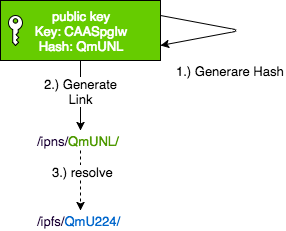
\includegraphics[width=0.7\textwidth]{img/ipns-1.png}
\caption[IPNS Step 1]{IPNS - Step 1}
\end{figure}
\newpage
\noindent
1.) To make this resolving process authenticated, the private key is used to sign a pointer object. The pointer object creates a link between the Public Key and the content. Three values are stored within this pointer object: The value (target hash), the key (public key hash) and a signature.\\
The pointer is another object in the IPFS Universe called IPRS Record. IPRS Records are stored on the Merkle DAG and can be used for authentication purposes.
\begin{figure}[H]
\centering
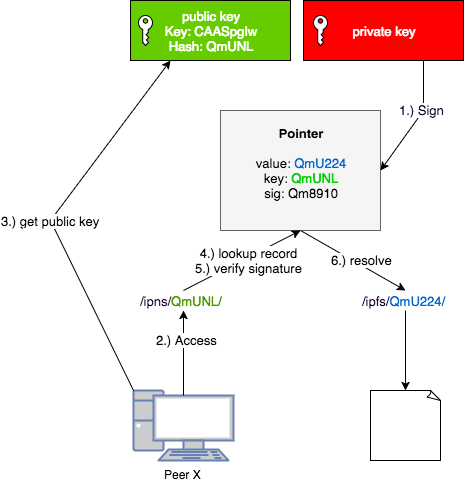
\includegraphics[width=0.7\textwidth]{img/ipns-2.png}
\caption[IPNS Step 2]{IPNS - Step 2}
\end{figure}
\noindent
2.) Peer X wants to resolv the IPNS link\\
3.) Gets the public key\\
4.) The peer will look for a pointer record in the DAG with the specific hash of the public key. \\
5.) The signature will be verified with the public key\\
6.) The peer will find the target hash value. This value will then be used to build the final ipfs link. \\ \\
If the content should be updated, only the target hash of the pointer needs to be changed. The ipns link stays the same.


\end{exmp}

\newpage
\subsection{DNS Links}
So far we created a static link to the content we want to present to the world. The systems works, but those ipns links are not very user friendly. We can use the existing DNS System to create user friendly links and map them to our IPNS links.\\
\begin{exmp} Map DNS to IPNS\\
We can add a TXT Record to the DNS Zone of our domain example: ipfs.io \cite{DNS}
\begin{center}
	dnslink="/ipns/QmWGb7PZmLb1TwsMkE1b8jVK4LGceMYMsWaSmviSucWPGG"
\end{center}
If we enter /ipns/ipfs.io the ipfs client will resolv the DNS TXT  entry and fetch the data from the ipns link above.
\end{exmp}



\chapter{Goals of IPFS}
The developers of IPFS  state: The Internet/Web of today has many issues.  The existing protocols we have today, have some major design issues or are not good enouth anymore to satisfy the needs of todays Web and his Users \cite{TodaysProblems}. In this chapter I will list the main problems the developers see and try to analyze if they can solve them.


\section{Offline functionality}
Imagine you are sitting with your colleagues at work. You all work together on a document. You are using a WebApplication to collaborate with each other. Suddenly the internet connection is lost. You are all sitting in the same network but you are unable to share your version of the document with the others. All the data needs to be synced with the backbone service for example Google Docs. and then down again to the other clients / your colleagues. The Applications should be able to talk to each other and shouldn't be dependant of a service somewhere in the internet.\\ \\
Thanks to the library libp2p, peers and their content can be detectet without any backbone service. The ipfs nodes can detect who owns which kind of data and request them. Webapplications can be served directly through ipfs. Once on the ipfs network the data is decentralized and can run without any central system. 

\section{Protocol}
The most used Protocol from the Internet Protocol Suite by far is HTTP. It follows the Server-Client communication model. The Client establishes a connection to one server, sends requests and get responses back from the server. Even if there are load balancing mechanisms in place it will be served by the by one host only.\\[0.3cm]
The alternative communication model would be Peer to Peer short. p2p. The Clients establishes a connection to mutlible ''peers'' which will serve the requested data. Every peer will deliver a fraction of the data. Those data ''pieces'' will be downloaded simultainously.

\newpage
\section{Permenancy}
I guess every person which used an Internet Browser before has seen a message like ''Error 404'' or ''Site not found''.
\begin{figure}[H]
\centering

\includegraphics[width=\textwidth]{img/github-404.png}
\caption[Github 404 Error Page]{Github 404 Error Page}
\end{figure}
\noindent
The specific content you tried to reach has been deletet or has been moved by the sites provider. All the links provided are now useless. Every day content gets moved around or is deleted forever. Sometimes its just a silly picture of a cat but mostly its data somebody actually would have needed.\\[0.3cm]
Nevertheless there are several companies already trying to solve this issue by archiving all the data available on the internet. The most well known would be ''Internet Archive'' with its ''Wayback Machine'' Webapplikation. They are using web crawlers to get the data and store them. The User is able to use theWayback Machine to view the webpage back then when the Internet Archive made a snapshot of it \cite{InternetArchive}. By October 2016 they managed to archive 273 billion webpages from over 361 million websites, which resulted in a data size of 15 Petabytes (15'000 Terabytes) \cite{InternetArchiveCount}.

\newpage

\section{Centralization \& Proxy}
Big data hosting companies like Google or Amazon own datacenters worldwide. Developer can buy the service from them to cluster their application data  and distrbute it all over the world. This ensures the availability of your Application even in case of a datacenter outage caused by a natural catastrophe or other technical issues. Those incidents aren't fictions and cost millions if they happen. Latest example, 28.02.2107 a site of the Amazon S3 System located in Northern Virginia gots unavailable. Thousands of webpages and webapplications stopped working. A Amazon technican wantet to remove a small subset of servers. He entered the command wrong and more servers than planned were removed. This led to an 4h outage of the hole Site \cite{AWSOutage}. Estimated cost 150 Million US Dollar \cite{AWSOutageCost}.\\\\
Clustering of data is not standard today. To make your data highly available is cost intensive. To achieve the same level of high availability cost effective without any kind of big service provider like Google is near impossible.\\\\
A second group of big data handlers are the so called CDNs. These Content Delivery Networks host data worldwide and act as a proxy for data requests. Services of these providers are used to bring content closer to the customers to reduce latency and download time.


\section{Security}

Man in the middle, armor the content not the tunnel

\section{Privacy \& Consumer Protection}
In these days one of the main concerns of social media platforms are privacy issues and hate messages. Those companies, for example Facebook and Twitter, are facing huge fines in several countries because goverments think they don't do enouth to protect their users. \cite{HateSpeech}. Content shared with a service in the internet, mostly stayes in the internet as its rapidly shared and distributed. If it's out there it's out there forerver. The content itself is hard to locate and remove. The data is adressed with links. The links or URL changes from hoster to hoster. If the affacted user tries to notify the hoster of the data, for example a picture with the intetion to damage the users reputation, it might alread be hosted by several other platforms.



\chapter{Todays Usage}
\section{Webhosting}
Static Webpages can be hosted easily on IPFS as they contain only static files like .css or .html.
Accordning to Juan Benet more than 100'000 webpages have been uploaded to IPFS \cite{ipfs-usage-web}.
\section{Software \& Private Cloud}
The IPFS protool has been bundled with the popular software FreeNas. Free NAS turns every computer into a NAS (Network attached Storage) \cite{freenas}. By leberaging the IPFS network the data of the NAS can be shared and distributed.

\section{Archive}
The developers of IPFS startet a new project to bring the content of Wikipedia on IPFS. This project was started due the recent blockade of the Wikipedia Website in Turkey on the 29.04.2017 \cite{turkeyblock}.

\section{Blockchain}
In the last years the blockchain technology gain alot of popularity. More and more projects have been introduced. Some of the well knowns are Bitcoin and Ethereum. Ethereum is a plattform to run applications, so called DAPPs, decentralized. One Example of DAPPs are Smart Contratcs. A Smart contratc is a piece of software which stores some rules for negotiating the terms of a contract. If the rules are fullfilled, the programm automatically executes the the agreed terms \cite{ether}. The blockchain is the wrong place to store big data \cite{blockchain-data}. Some companies discovered IPFS to outsoruce tha data. The data is placed on the IPFS Network and only the hash  / link is stored in th blockchain.

\chapter{Conclusion}


\chapter{Disclaimer-Notice}



\begin{thebibliography}{1}
\bibitem{specs} \url{https://github.com/ipfs/specs}, 29.04.2017
\bibitem{IPFSBasics} \url{https://github.com/ipfs/ipfs}, 24.07.2017
\bibitem{LinkedIn} \url{https://www.linkedin.com/in/jbenetcs/}, 28.04.2017
\bibitem{Tribute} \url{https://www.youtube.com/watch?v=HUVmypx9HGI} 4:30, 22.04.2017
\bibitem{JCR} \url{http://www.internetsociety.org/internet/what-internet/history-internet/brief-history-internet}, 22.04.2017
\bibitem{TodaysProblems} \url{https://ipfs.io/}, Sector: The web of tomorrow needs IPFS today, 22.04.2017
\bibitem{InternetArchive} \url{https://en.wikipedia.org/wiki/Internet_Archive}, 22.04.2017
\bibitem{InternetArchiveCount} \url{https://blog.archive.org/2016/10/23/defining-web-pages-web-sites-and-web-captures}, 22.04.2017
\bibitem{AWSOutage} \url{https://aws.amazon.com/message/41926/}, 23.04.2017
\bibitem{AWSOutageCost} \url{http://www.npr.org/sections/thetwo-way/2017/03/03/518322734/amazon-and-the-150-million-typo}, 23.04.2017
\bibitem{HateSpeech} \url{https://www.nytimes.com/2017/03/14/technology/germany-hate-speech-facebook-tech.html?_r=0}, 23.04.2017
\bibitem{HTTPAdressing} \url{https://www.w3.org/Addressing/HTTPAddressing.html}, 23.04.2017 
\bibitem{PeerID}\url{https://github.com/ipfs/faq/issues/238}, 24.04.2017
\bibitem{hasfunction} \url{https://github.com/ipfs/faq/issues/22}, 30.04.2017
\bibitem{multihash} \url{https://github.com/jbenet/random-ideas/issues/1}, 24.04.2017
\bibitem{Encoding} \url{https://github.com/ipfs/faq/issues/22}, 30.04.2017
\bibitem{Encryption} \url{https://github.com/ipfs/faq/issues/116}, 30.04.2017
\bibitem{EncryptionManual} \url{https://github.com/ipfs/faq/issues/4}, 30.04.2017
\bibitem{bitswap} \url{https://github.com/ipfs/specs/tree/master/bitswap}, 29.04.2017
\bibitem{fileblock} \url{https://github.com/ipfs/examples/tree/master/examples/data}, 29.04.2017
\bibitem{fileblock2} \url{https://medium.com/@ConsenSys/an-introduction-to-ipfs-9bba4860abd0}, 29.04.2017
\bibitem{bitswapstrategy} \url{https://github.com/ipfs/faq/issues/47}, Q: but bitswap says..., 29.04.2017
\bibitem{Routing} \url{https://github.com/ipfs/faq/issues/48}, 29.04.2017
\bibitem{copyright}\url{https://www.reddit.com/r/ipfs/comments/3m351b/discussion_permanent_content_dmca_and_illegal/?st=j24nd4on&sh=86fd55ce}
\bibitem{Whitepaper} Whitepaper
\bibitem{libp2pissues} \url{https://www.infoq.com/presentations/data-ipfs-ipld}, 15min
\bibitem{libp2pnoip} \url{https://github.com/libp2p/specs/blob/master/3-requirements.md} 
 \bibitem{dht-provide} \url{https://github.com/ipfs/go-ipfs/issues/1396}
\bibitem{DNS} \url{https://news.ycombinator.com/item?id=10229481} 14.05.2017
\bibitem{ipfs-usage-web} \url{}
\bibitem{freenas} \url{http://www.freenas.org/blog/announcing-freenas-10-alpha/}
\bibitem{turkeyblock} \url{https://ipfs.io/blog/24-uncensorable-wikipedia/}
\bibitem{ether}
\bibitem{blockchain-data} \url{http://www.coindesk.com/ethereum-meets-zcash-why-ipfs-plans-a-multi-blockchain-browser/}

\end{thebibliography}


\printglossaries

\listoffigures
%https://github.com/multiformats/multihash/blob/master/hashtable.csv


\end{document}